\documentclass[tikz,border=4pt]{standalone}
\usepackage{libertinus}
\usepackage{amsmath}
\usetikzlibrary{
  arrows.meta,
  backgrounds,
  calc,
  decorations.markings,
  fit,
  positioning
}

\definecolor{accent}{RGB}{38,103,115}
\definecolor{softgray}{RGB}{244,245,246}
\definecolor{midgray}{RGB}{123,128,132}

\tikzset{
  >={Latex[length=2.2mm,width=1.5mm]},
  flow/.style={-Latex,semithick,draw=black!72},
  accent flow/.style={-Latex,semithick,draw=accent},
  box/.style={
    draw=black!68,
    fill=softgray,
    rounded corners=1.2pt,
    align=center,
    inner xsep=5pt,
    inner ysep=4pt
  },
  accent box/.style={
    draw=accent,
    fill=accent!8,
    rounded corners=1.2pt,
    align=center,
    inner xsep=5pt,
    inner ysep=4pt
  },
  point/.style={circle,draw=black!75,fill=white,inner sep=1.7pt},
  accent point/.style={circle,draw=accent,fill=accent!10,inner sep=1.7pt},
  tinylabel/.style={font=\scriptsize,align=center},
  smalllabel/.style={font=\small,align=center},
  panel/.style={draw=black!28,rounded corners=2pt,inner sep=6pt}
}


\tikzset{
  old arc/.style={draw=black!55,semithick},
  selected arc/.style={draw=black,very thick},
  new arc/.style={draw=accent,very thick,densely dashed},
  value/.style={circle,draw=black!75,fill=white,minimum size=4mm,inner sep=0pt},
  first point/.style={value,rectangle,draw=black,thick,fill=softgray},
  pending/.style={value,dashed,text=black!65},
  heading/.style={font=\small\bfseries,anchor=west},
  note/.style={anchor=west,inner sep=0pt}
}
\newcommand{\framepanel}[1]{%
  \draw[black!28,rounded corners=2pt] (.03,1.95) rectangle (5.97,-3.13);
  \node[heading] at (.15,1.65) {#1};
}
\newcommand{\arcs}[1]{%
  \draw[black!45] (.58,0) -- (5.42,0);
  \draw[old arc] (1,0) arc[start angle=180,end angle=0,x radius=.5,y radius=.55];
  \draw[old arc] (3,0) arc[start angle=180,end angle=0,x radius=1,y radius=.77];
  \draw[#1] (1,0) arc[start angle=180,end angle=360,x radius=2,y radius=.99];
}
% Keep the point indices in a separate row below the arcs.
\newcommand{\points}[1]{%
  \foreach \x/\idx in {1/3,2/4,3/1,5/2}{
    \ifnum\x=3 \node[first point] (p3) at (3,0) {3};
    \else \node[value] (p\x) at (\x,0) {\x}; \fi
    \node at (\x,-1.33) {$z_{\idx}$};
  }
  \ifnum#1>0
    \ifnum#1=1 \node[pending] at (4,0) {4};
    \else \node[value] at (4,0) {4}; \fi
    \node at (4,-1.33) {$z_5$};
  \fi
}

\begin{document}
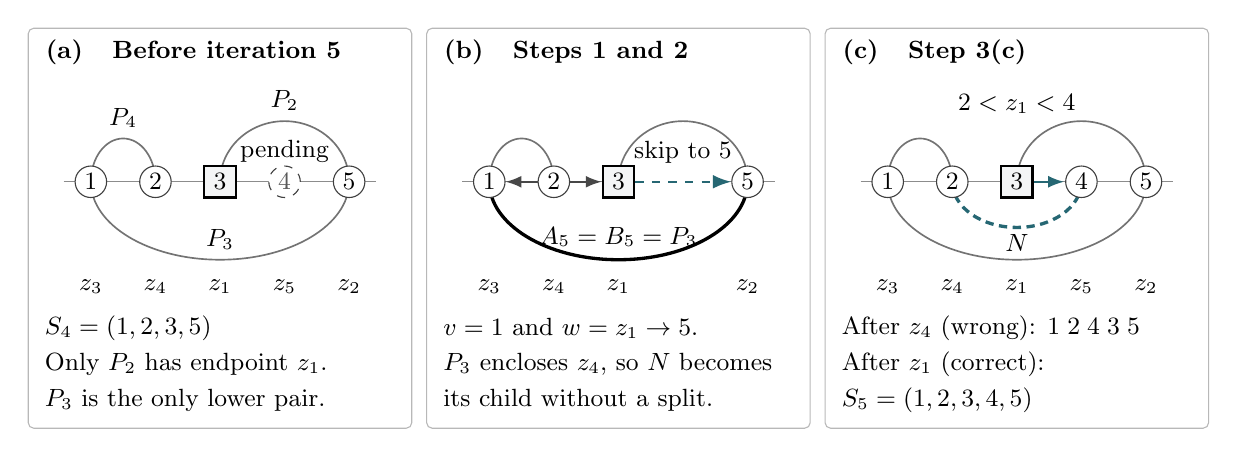
\begin{tikzpicture}[x=.82cm,font=\small]
  \begin{scope}
    \framepanel{(a)\quad Before iteration 5}
    \arcs{old arc}
    \points{1}
    \node at (1.5,.81) {$P_4$};
    \node at (4,1.03) {$P_2$};
    \node at (4,.39) {pending};
    \node at (3,-.73) {$P_3$};
    \node[note] at (.28,-1.86) {$S_4=(1,2,3,5)$};
    \node[note] at (.28,-2.32) {Only $P_2$ has endpoint $z_1$.};
    \node[note] at (.28,-2.78) {$P_3$ is the only lower pair.};
  \end{scope}
  \begin{scope}[xshift=5.06cm]
    \framepanel{(b)\quad Steps 1 and 2}
    \arcs{selected arc}
    \points{0}
    \draw[flow] (p2.west) -- (p1.east);
    \draw[flow] (p2.east) -- (p3.west);
    \draw[accent flow,thick,dashed,preaction={draw=white,solid,line width=2pt}] (p3.east) -- (p5.west);
    \node at (4,.37) {skip to 5};
    \node at (3,-.70) {$A_5=B_5=P_3$};
    \node[note] at (.28,-1.86) {$v=1$ and $w=z_1\to 5$.};
    \node[note] at (.28,-2.32) {$P_3$ encloses $z_4$, so $N$ becomes};
    \node[note] at (.28,-2.78) {its child without a split.};
  \end{scope}
  \begin{scope}[xshift=10.12cm]
    \framepanel{(c)\quad Step 3(c)}
    \arcs{old arc}
    \draw[new arc] (2,0) arc[start angle=180,end angle=360,x radius=1,y radius=.58];
    \points{2}
    \draw[accent flow] (p3.east) -- (3.73,0);
    \node at (3,-.78) {$N$};
    \node at (3,.99) {$2<z_1<4$};
    \node[note] at (.28,-1.86) {After $z_4$ (wrong): $1\;2\;4\;3\;5$};
    \node[note] at (.28,-2.32) {After $z_1$ (correct):};
    \node[note] at (.28,-2.78) {$S_5=(1,2,3,4,5)$};
  \end{scope}
\end{tikzpicture}
\end{document}
